\chapter{Combined Topological and Algebraic Structures}


\begin{summary}[A useful trick]
	Let $ x,y\in \R $. Then we want to show for $ p\in (0,1) $ we have
	\[ \abs{x+y}^p \leq \abs{x}^p + \abs{y}^p. \]
	To see this let $ \beta = 1-p $. Then we can write
	\[ \abs{x+y}^p = \abs{x+y}^{1-\beta} = \frac{\abs{x+y}}{\abs{x+y}^\beta} \leq \frac{\abs{x}}{\abs{x+y}^\beta} + \frac{\abs{y}}{\abs{x+y}^\beta} \leq \frac{\abs{x}}{\abs{x}^\beta} + \frac{\abs{y}}{\abs{y}^\beta} = \abs{x}^p + \abs{y}^p. \]
\end{summary}

\begin{summary}
	\[ \norm{x} = \int_{0}^{1} \abs{x(t)}^p dt < \infty \]
	is a not a norm but $ d(x,y) = \norm{x-y} $ is a metric.
\end{summary}

\begin{summary}[Not norm but metric!]
	There are functions $ \norm{\cdot}:V \to\R $ defined on a vector space, that are not norm, but $ d(x,y) = \norm{x-y} $ is a metric. It is enough for a function $ \norm{\cdot} $ to be non-negative, and positive definite, and satisfy the triangle inequality and have $ \norm{x}=\norm{-x} $. Then $ d(x,y) =\norm{x-y} $ will be a metric. There is no need for homogeneity condition.
\end{summary}

\begin{summary}
	Any metric $ d $ on a vector space $ V $ comes from a function $ \norm{x} $ that need to satisfy all norm properties except for the homogeneity condition. And it also need to satisfy $ \norm{x} = \norm{-x} $. See \autoref{prob:allMetricsOnLinearSpace}.
\end{summary}


\begin{summary}[A common confusion]
	Note that the collection $ B = \set{e_1,e_2,e_3,\cdots} $ is not a basis for $ \ell_2(\R) $. That is because the sequences with infinite support can not be written as a finite linear combination of elements in the basis. But by the Zorn's lemma, every vector space does contain a Hamel basis. And in this case, this Hamel basis exists but is not constructive.
\end{summary}


\begin{summary}[A very dangerous intuition]
	In studying the theory of the convergence of series of real numbers, one might build the following mental picture
	% https://q.uiver.app/#q=WzAsNSxbMSwwLCJcXHRleHR7Q29udmVyZ2VudCBzZXJpZXN9Il0sWzAsMSwiXFx0ZXh0e2NvbmRpdGlvbmFseSBjb252ZXJnZW50fSJdLFsyLDEsIlxcdGV4dHt1bmNvbmRpdGlvbmFseSBjb252ZXJnZW50fSJdLFsyLDIsIlxcdGV4dHthYnNvbHV0ZWx5IGNvbnZlcmdlbnR9Il0sWzAsMiwiXFx0ZXh0e25vdCBhYnNvbHV0ZWx5IGNvbnZlcmdlbnR9Il0sWzAsMV0sWzAsMl0sWzIsM10sWzEsNF1d
	\[\begin{tikzcd}
		& {\text{Convergent series}} \\
		{\text{conditionaly convergent}} && {\text{unconditionaly convergent}} \\
		{\text{not absolutely convergent}} && {\text{absolutely convergent}}
		\arrow[from=1-2, to=2-1]
		\arrow[from=1-2, to=2-3]
		\arrow[from=2-1, to=3-1]
		\arrow[from=2-3, to=3-3]
	\end{tikzcd}\]
	Howerver, this is not true in a general metric space. I.e. in general it is possible to come up with an unconditionaly convergent series that is not absolutely convergent! In the note in page 227 of the text book, we read that Dvoretzky and Rogers have proved that an unconditionaly convergent series is absolutely convergent if and only if the space is finite dimensional. This givens us enough hint to come up with our own example. Because and unconditional convergence is absolutely convergent if and only if the space is finite dimensional, it follows that it is some property of infinite dimension that can lead to an unconditional convergent series that is not absolutely convergent. One possible property of the infinite dimension that we can exploit is the escape of the mass to the infinity. Consider the sequence $ \set{x_n} $ in $(C(\R),\norm{\cdot}) $ where one particular $ x_n $ is shown as below
	\begin{center}
	
	
	\tikzset{every picture/.style={line width=0.75pt}} %set default line width to 0.75pt        
	
	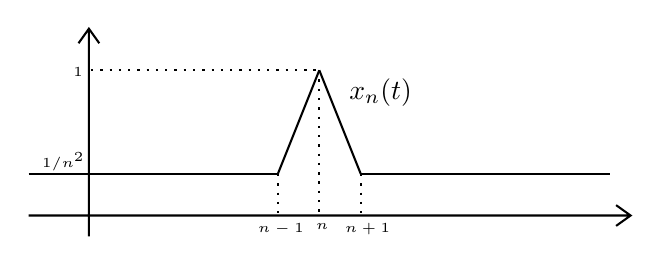
\begin{tikzpicture}[x=0.75pt,y=0.75pt,yscale=-1,xscale=1]
		%uncomment if require: \path (0,300); %set diagram left start at 0, and has height of 300
		
		%Shape: Axis 2D [id:dp1663102831517027] 
		\draw  (100,160) -- (390,160)(129,70) -- (129,170) (383,155) -- (390,160) -- (383,165) (124,77) -- (129,70) -- (134,77)  ;
		%Straight Lines [id:da8094250901048163] 
		\draw    (100,140) -- (220,140) ;
		%Straight Lines [id:da3926524751184308] 
		\draw    (220,140) -- (240,90) ;
		%Straight Lines [id:da9345956516168132] 
		\draw    (260,140) -- (240,90) ;
		%Straight Lines [id:da2510520175171027] 
		\draw    (260,140) -- (380,140) ;
		%Straight Lines [id:da6251110538749508] 
		\draw  [dash pattern={on 0.84pt off 2.51pt}]  (240,90) -- (240,160) ;
		%Straight Lines [id:da5544158951216948] 
		\draw  [dash pattern={on 0.84pt off 2.51pt}]  (220,140) -- (220,160) ;
		%Straight Lines [id:da20393290290096278] 
		\draw  [dash pattern={on 0.84pt off 2.51pt}]  (260,140) -- (260,160) ;
		%Straight Lines [id:da6458699328315521] 
		\draw  [dash pattern={on 0.84pt off 2.51pt}]  (130,90) -- (240,90) ;
		
		% Text Node
		\draw (120,87.4) node [anchor=north west][inner sep=0.75pt]  [font=\tiny]  {$1$};
		% Text Node
		\draw (209,162.4) node [anchor=north west][inner sep=0.75pt]  [font=\tiny]  {$n-1$};
		% Text Node
		\draw (251,162.4) node [anchor=north west][inner sep=0.75pt]  [font=\tiny]  {$n+1$};
		% Text Node
		\draw (237,162.4) node [anchor=north west][inner sep=0.75pt]  [font=\tiny]  {$n$};
		% Text Node
		\draw (253,92.4) node [anchor=north west][inner sep=0.75pt]    {$x_{n}( t)$};
		% Text Node
		\draw (105,128.4) node [anchor=north west][inner sep=0.75pt]  [font=\tiny]  {$1/n^{2}$};
		
		
	\end{tikzpicture}
\end{center}
	The sequence of partial sums in $ \sum_n x_n $ is monotone and bounded (an upper bound is 5. That is because at each $ t $, the series for that value is $ \sum_n 1/n^2 $ with except one term replaced by 1. So the worst that can happen is that keep all the terms and add one to the final infinite sequence. So an upper bound would be $ \sum_n 1/n^2 + 1 $.)
\end{summary}

\newpage


\section{Problems}
\subsection{Normed Linear Spaces}
\begin{problem}
	Show that the norm $ \norm{\cdot} $ considered as a mapping of a normed linear space $ X $ into the reals is continues.
\end{problem}

\begin{solution}
	We use the reverse triangle inequality, i.e. for $ x,y \in X $ we have
	\[ \abs{\norm{x} - \norm{y}} \leq \norm{x-y}. \]
	Let $ \epsilon>0 $ given and let $ d(x,y)=\norm{x-y}<\epsilon $. Then it implies that
	\[ d(\norm{x},\norm{y}) = \abs{\norm{x} - \norm{y}} \leq \norm{x-y} <\epsilon. \]
	So $ \norm{\cdot} $ is continuous.
\end{solution}
\begin{remark}
	In the problem above we implicitly assume that the real line (co-domain of the norm function) is has the topology induced by $ \abs{\cdot} $.
\end{remark}

\begin{problem}
	Show that the addition and scalar multiplications in a vector space are continuous.
\end{problem}
\begin{solution}
	Let $ \cdot\ + \cdot\ : X\times X \to X $ denote the addition operation in a vector space. We assume that $ X $ has the topology induced by $ \norm{\cdot} $ and $ X\times X $ has the topology induced by $ \norm{(x,y)} = \norm{x} + \norm{y} $. Let $ (a,u),(b,v)\in X\times X $. Let $ \epsilon>0 $ such that $ d((a,u),(b,v)) = \norm{(a-b,v-u)} = \norm{a-b} + \norm{v-u} < \epsilon $. Then we can write
	\[ d(a+u,b+v) = \norm{a+u-b-v} \leq \norm{a-b}+\norm{u-v} = d((a,u),(b,v))<\epsilon. \]
	
	For the scalar multiplication, let $ \cdot: F\times X $ denote the scalar multiplication. We assume $ F $ is $ \R $ with the usual topology. Then 
	\[ \norm{\alpha u - \beta v} = \norm{\alpha u \pm \alpha v - \beta v} \leq \norm{\alpha(u-v)} + \norm{v(\alpha-\beta)} = \abs{\alpha}\norm{u-v} + \abs{\alpha-\beta}\norm{v}. \]
	Let $ \epsilon >0 $ given and choose $ \norm{u-v} < \epsilon/\alpha $ and $ \abs{\alpha-\beta}<\epsilon/\norm{v} $. So when $ d((\alpha,u),(\beta,v)) = \norm{u-v}+\abs{\beta-v} < \delta $ where $ \delta = \epsilon/\alpha + \epsilon/\norm{v} $ we will have
	\[ \norm{\alpha u - \beta v} < \epsilon. \] 
	So the scalar multiplication is continuous. Note that the choice of $ \delta $ depends on $ v $. So the scalar multiplication is \textbf{not} uniformly continuous.
\end{solution}

\begin{problem}
	Characterize all possible norms on the real line $ \R $, where $ \R $ is considered a real linear space. Ont eh complex plane $ \C$, where $ \C  $ is considered as a complex linear space. Show that $ \C $ may have other norms when it is considered as a real linear space. 
\end{problem}
\begin{solution}
	We know that $ \abs{\cdot}:\R\to\R $ is a norm on $ \R $. Let $ f(x) $ be any other norm on this space. Then define $ g(x) = f(x)/\abs{x} $ for $ x\neq0 $. For any $ \alpha\in\R  $ we will have
	\[ g(\alpha x) = g(x) \quad \forall \alpha,x\in\R . \]
	This implies that $ g $ is a constant function. Because, let $ x,y\in \R\backslash\set{0} $ then $ g(x) - g(y) = g(x) - g(\beta x) = g(x) - g(x) = 0  $ where $ \beta = y/x $. So $ f(x) = \alpha \abs{x} $ where $ g(x) \equiv \alpha $. So all of the norms on $ \R $ are of the form $ \norm{x} $.
	
	On the complex plane $ \C $ as a vector space over $ \C $ we define the norm as
	\[ \norm{u} = \sqrt{u\conj{u}}. \]
	Similar to above, define $ g(u) = f(u)/\norm{u} $ where $ f(u) $ is any other norm. Then we will have $ g(\alpha u) = g(u) $ for all $ u,\alpha \in \C $. Let $ u,v\in \C $. Then $ \exists \alpha\in \C $ such that $ u=\alpha v $ (this is only true if $ \C $ is a vector space over $ \C $). So $ g(u) - g(v) = g(u) - g(\alpha u) = 0 $. So $ g $ is a constant function. So we conclude that every norm in $ (\C,\C) $ is in the form of $ \abs{\alpha} \norm{\cdot} $ for $ \alpha\in \C $.
	
	However, if we consider $ \C $ as a vector space over $ \R $, then there are other norms different from the form above. For instance $ \norm{u} = \sqrt{\Im{u}^2 + \Re{u}^2} $ is a norm.
\end{solution}


\begin{problem}
	Let $ (X,\norm{\cdot}) $ be a normed linear space and let $ S_r = \set{x:\norm{x}=r} $ where $ r>0 $. Assume that $ X\neq \set{0} $. Show that $ (X,\norm{\cdot}) $ is a Banach space if and only if the metric space $ (S_r,\norm{\cdot}) $ is complete for some $ r>0 $.
\end{problem}

\begin{solution}
	First we show if $ S_r $ is complete then $ X $ is complete. Let $ \set{x_n} $ be a Cauchy sequence in $ X $. There are two cases: The first case is that $ x_n $ gets arbitrarily close to the origin, and the second case is that for large enough $ n $, $ x_n $ is uniformly away from the origin. Since the sequence is Cauchy, these are the only two possible cases. For the first case we have $ \forall \epsilon>0 $, $ \exists N > 0 $ such that $ \forall n>N $ we have $ \norm{x_n}<\epsilon $, we have $ x_n\to 0 \in X $, thus converges. The second case is that for $ n $ large enough, the sequence is uniformly away from the origin. For this case case, where $ \exists\epsilon>0 $ and $ \exists N>0 $ such that $ \norm{x_n}>0 $. We map the sequence $ \set{x_n} $ to a sequence $ \set{y_n} \subset S_r $ via
	\[ y_n = \frac{rx_n}{\norm{x_n}}. \]
	Since this map is continuous (using the fact that every Cauchy sequence is bounded, so is $ \set{x_n} $), $ y_n $ is also Cauchy, thus it converges: $ y_n\to y\in S_r $. Using the continuity of $ \norm{\cdot} $, the sequence $ \set{\norm{x_n}}\subset\R $ is Cauchy, thus it converges: i.e. $ \norm{x_n} \to a\in \R $. We claim $ x_n \to x = ay/r $. Because if we assume other wise, then $ \set{y_n} $ is not converging to $ y $, which is against our hypothesis.
	
	For the other direction, we assume $ X $ is Banach and we want to conclude $ S_r $ is complete. Let $ \set{x_n} \subset S_r $ be a Cauchy sequence. Since $ S_r\subset X $, then $ \set{x_n} $ is also a Cauchy sequence in $ X $, hence converges to $ x \in X $. We want to show that $ \norm{x} = r $, thus belongs to $ S_r $. To show this we use the fact that $ \norm{\cdots} $ is a continuous map. So since $ \norm{x_n} = r $ for all $ n $, it follows that $ \norm{x} = 1 $ as well. 
\end{solution}

\begin{problem}
	Let $ p $ satisfy $ 0<p<1 $ and consider the space $ L_p[0,1] $ of all functions with 
	\[ \norm{x} = \int_0^1 \abs{x(t)}^p dt < \infty. \]
	Show that $ \norm{x} $ is not a norm on $ L_p[0,1] $. Show that $ d(x,y) = \norm{x-y} $ is a metric on $ L_p[0,1] $. Hint: Note that if $ 0\leq\alpha\leq 1 $ then $ \alpha<\alpha^p \leq 1 $.
\end{problem}
\begin{solution}
	The fact that $ \norm{\cdot} $ as defined above is not a norm follows from the fact that it is not homogeneous. I.e. for $ \alpha\in\R $  we have $ \norm{\alpha x} = \abs{\alpha}^p \norm{x} $. But $ d(x,y) = \norm{x-y} $ is a metric. That is because it satisfies the metric properties, in particular $ d(x,y) \leq d(x,z) + d(z.y) $. See the following remark for the triangle inequality.
\end{solution}
\begin{remark}
	Let $ x,y\in \R $. Then we want to show for $ p\in (0,1) $ we have
	\[ \abs{x+y}^p \leq \abs{x}^p + \abs{y}^p. \]
	To see this let $ \beta = 1-p $. Then we can write
	\[ \abs{x+y}^p = \abs{x+y}^{1-\beta} = \frac{\abs{x+y}}{\abs{x+y}^\beta} \leq \frac{\abs{x}}{\abs{x+y}^\beta} + \frac{\abs{y}}{\abs{x+y}^\beta} \leq \frac{\abs{x}}{\abs{x}^\beta} + \frac{\abs{y}}{\abs{y}^\beta} = \abs{x}^p + \abs{y}^p. \]
\end{remark}



\begin{problem}
	Define
	\begin{align*}
		\sigma_n(f) = \sup\set{\abs{f(t)}: \abs{t}\leq n}, \\
		\rho_n(f) = \min(1,\sigma_n(f)),\\
		\norm{f} = \sum_{n=1}^{\infty} 2^{-n}\rho_n(f),
	\end{align*}
	where $ f\in C(-\infty,\infty) $.
	
	\begin{enumerate}[(a)]
		\item Show that $ \sigma_n(f) $ is a pseudo-norm on on $ C(-\infty,\infty) $.
		\item Show that $ \rho_n(f) $ and $ \norm{f} $ are not norms.
		\item Show that $ d(f,g) = \norm{f-g} $ is a metric on $ C(-\infty,\infty) $.
		\item Show that $ d(f_n,f) \to 0 $ as $ n\to\infty $ if and only if $ f_n(t) \to f(t)$ uniformly on compact sets in $ -\infty<t<\infty $.
	\end{enumerate}
\end{problem}


\begin{solution}
	\begin{enumerate}[(a)]
		\item For any choice of $ n $, the function
		\[ f(t) = \begin{cases}
			0 \quad \abs{t}<n,\\
			x-n \quad t\geq n,\\
			-x-n \quad t\leq n
		\end{cases}, \]
		and the origin both has norm zero.
		
		\item Let $ f \equiv 5 $. Then $ \sigma_n(f) = 5 $ for all $ n\in\N $ and $ \rho_n(f) = 1 $ for all $ n\in \N $. For all $ \alpha \geq 1/5 $ we also have $ \rho_n(\alpha f) = \rho_n(f) $. Thus $ \rho $ is not homogeneous. So it is not a norm. For the same reason, $ \norm{\cdot} $ is not a norm.
		
		\item $ d(x,y) = \norm{x-y} $ satisfies all of the metric properties. In particular, for the triangle inequality we have
		\[ \sigma_n(f+g) = \sup\set{\abs{f+g}} \leq \sup\set{\abs{f}+\abs{g}}\leq \sup\set{f} + \sup\set{g} = \sigma_n(\abs{f}) + \sigma_n(\abs{g}), \]
		where $ \sup\set{\abs{f}} $ is used as a short notation for $ \sup\set{\abs{f(t)}:\abs{t}<n}. $. Furthermore, we know that $ \min(1,a+b) $ for $ a,b>0 $ we have $ \min(1,a+b) \leq \min(1,a) + \min(1,b)  $. Because there are 4 cases: $ a,b<1 $ with their sum $ a+b<1 $, $ a,b<1 $ with $ a+b> 1 $, $ a,b>1 $, and $ a<1<b $. In all of these cases the inequality holds. Furthermore, we have
		\[ \norm{f+g}  = \sum_{n=1}^{\infty} 2^{-n}\rho_n(f+g) \leq \sum_{n=1}^{\infty}2^{-n}\rho_n(f) + \sum_{n=1}^{\infty}2^{-n}\rho_n(g).  \]
		This is true because $ \rho_n(f+g)\leq 1 $ and $ \rho_n(f+g) \leq \rho_n(f) + \rho_n(g) \leq 2 $. So the $ \sum 2^{-n}\rho_n(f+g) $ is absolutely convergent. This $ \sum 2^{-n}\rho_n(f+g) \leq \sum 2^{-n}(\rho_n(f) + \rho_n(g)) \leq \sum 2^{-n}\rho_n(f) + \sum 2^{-n}\rho_n(g).  $
		
		
		\item Still thinking!
	\end{enumerate}
\end{solution}



\begin{problem}
	\label{prob:allMetricsOnLinearSpace}
	Let $ X $ be a linear space and let $ \norm{x} $ be a real-valued function defined on $ X $. Show that $ d(x,y) = \norm{x-y} $ is a metric if and only if $ \norm{x} $ satisfies (N1), (N2), (N4), and $ \norm{x} = \norm{-x} $ for all $ x\in X $.
\end{problem}

\begin{solution}
	Assume $ \norm{x} $ satisfies (N1), (N2), (N4), and $ \norm{x} = \norm{-x} $. Then $ d(x,y) = \norm{x-y} $ is positive (from N1) and $ d(x,y) = 0 $ iff $ x=y $ (from positive definiteness of $ \norm{\cdot} $), and $ d(x,y) = d(y,x) $ from $ \norm{x} = \norm{-x} $. $ d(x,y) \leq d(x,z) + d(z,y)  $ from the triangle inequality for $ \norm{\cdot} $. 
	
	Now assume $ d(x,y)  = \norm{x-y} $ is a metric. $ \norm{x} = d(x,0) \leq 0 $, so $ \norm{\cdot}$ is non-negative. Also $ d(x,y) = d(y,x) $ implies $ \norm{x} = \norm{-x} $. Furthermore, in $ d(x,y) \leq d(x,z) + d(z,y) $, let $ z=0 $, and we will recover $ \norm{x-y} \leq \norm{x} + \norm{-y} $. Let $ \tilde{y} = -y $. Then $ \norm{x+\tilde{y}} \leq \norm{x} + \norm{\tilde{y}} $, hence the triangle inequality for the norm. Lastly, for the positive definiteness, Let $ \norm{x} = 0 $. Since $ \norm{x} = \norm{x-0} = d(x,0) $, it follows that $ d(x,0) = 0 $. Thus $ x=0 $ from metric properties. Also if $ x=0 $, then $ \norm{0} = \norm{0-0} = d(0,0) = 0 $.
\end{solution}


\begin{problem}
	Let $ (X,\norm{\cdot}) $ be a normed linear space and let $ \set{x_n} $ be a sequence in $ X $ with $ x=\lim_{n\to\infty} x_n $. Assume that $ \norm{x_n-y} \leq a $ for all $ n $. Show that $ \norm{x-y} \leq a $. 
\end{problem}
\begin{solution}
	Since $ x_n \to x $, from the continuity of the addition in vector space, it also follows that $ x_n -y \to x-y $. From continuity of $ \norm{\cdot} $ it follows that the real sequence $ \set{\norm{x_n-y}} $ converges to $ \norm{x-y} $. Since all elements of the real sequence $ \norm{x_n-y} $ is less than or equal to $ a $, then the for the limit will will have $ \norm{x-y} \leq a $. This property for the real sequences can be shown with a simple proof by contradiction.
\end{solution}


\begin{problem}
	Show that a Hamel basis for a Banach space is either finite or uncountably infinite. (Completeness is important for this. Use Exercise 17, section 3.13).
\end{problem}

\begin{solution}
	Let $ X $ be a Banach space with countable Hamel basis, i.e. $ B = \set{e_1,e_2,\cdots} $. Consider $ A_n = \vspan{e_1,e_2,\cdots,e_n} $ (see the remark below). Then since $ \forall v\in X $, $ v $ is a finite linear combination of some basis vectors, it follows that $ v \in \vspan{A_n} $ for some $ n $. Thus
	\[ X = \cup_{n\in \N} A_n. \] 
	We know that every finite dimensional vector space is closed. But non of $ A_n $ contains an open ball (hence an open set), (otherwise with translation and scaling this implies $ A_n $ contains the unit ball, which implies that $ A_n = X $). Using the result of Exercise 17, section 3.13 we conclude that $ X $ is not complete, which is a contradiction to the assumption that $ X $ is a Banach space. 
\end{solution}
\begin{remark}
	Note that one can not write $ A_n = \vspan{e_n} $ and claim $ X = \cup_n A_n $. This is not true! Instead, one can write $ A_n = \vspan{e_1,\cdots,e_n} $. Then each $ A_n $ is finite dimensional, and since $ B $ is a Hamel basis, any $ v\in X $ is in some $ A_n $. Thus $ X = \cup_n A_n $. Note that if one writes $ X = \cup_{A\in \mathcal{I}}A $, where $ \mathcal{I} $ is the set of all finite dimensional subspaces of $ X $, one should note that the union is on uncountably infinite collection of sets.
\end{remark}

\begin{problem}[{\color{orange} Important}]
	Let $ X $ denote the collection of all sequences $ x=  (x_1,x_2,\cdots) $ of complex numbers and define
	\[ \norm{x} = \sum_{n=1}^{\infty}2^{-n}\min(1,\abs{x_n}). \]
	\begin{enumerate}[(a)]
		\item Is $ \norm{\cdot} $ a norm on $ X $?
		\item Does $ \norm{x-y} $ define a metric on $ X $? If so, explain the meaning of $ \norm{x^{(n)}-x}\to 0 $ as $ n\to0 $.
	\end{enumerate}
\end{problem}
\begin{solution}
	\begin{enumerate}[(a)]
		\item No. Let $ x = (1,1,\cdots) $. Then $ \norm{x} = 2 $. However, $ \norm{2x} = 2 \neq 2\norm{x} $. So $ \norm{\cdot} $ is not homogeneous, hence not a norm.
		
		\item Yes $ \norm{x-y} $ does define a metric. Symmetry and positive definiteness comes from the properties of $ \abs{\cdot} $. For the triangle inequality, it follows from
		\[ \min(1,\abs{a+b}) \leq \min(1,\abs{a} + \abs{b}) \leq \min(1,\abs{a}) + \min(1,\abs{b}).  \]
		
		The meaning of convergence in this metric is similar to the convergence of real numbers (or complex numbers) when expanded in their decimal expansion. 
 	\end{enumerate}
\end{solution}

\begin{problem}[\color{orange} Important]
	Give and example of a metric $ d $ on a linear space such that $ d(x,0) $ is not a norm.
\end{problem}
\begin{solution}
	First consider the following Lemma
	\begin{lemma}
		for $ 0<p<1 $ one has
		\[ \abs{expression}^p \leq \abs{x}^p + \abs{y}^p. \]
		\begin{proof}
			Let $ \beta = 1-p $. Then
			\[ \abs{x+y}^p = \frac{\abs{x+y}}{\abs{x+y}^{\beta}}\leq \frac{\abs{x}}{\abs{x+y}^\beta} + \frac{\abs{y}}{\abs{x+y}^\beta} \leq \frac{\abs{x}}{\abs{x}^\beta} + \frac{\abs{y}}{\abs{y}^\beta} = \abs{x}^p + \abs{y}^p. \]
		\end{proof}
		So $ d(x,y) = \abs{x-y}^p $ is a metric. However, $ d(x,0) = \abs{x}^p $ is not a norm as it is not homogeneous.
 	\end{lemma}
\end{solution}


\begin{problem}
	A real-valued function $ f $ defined on a linear space $ X $ is said to be convex, if
	\[ f(\alpha x + \beta y) \leq \alpha f(x) + \beta f(y), \]
	for all $ 0\leq \alpha,\beta \leq 1 $ with $ \alpha + \beta = 1 $. Show that a norm is a convex function.
\end{problem}
\begin{solution}
	It follows from the homogeneity of the norm and the triangle inequality.
	\[ \norm{\lambda x + (1-\lambda)y} \leq \norm{\lambda x} + \norm{(1-\lambda)y} = \abs{\lambda} \norm{x} + \abs{1-\lambda}\norm{y} = \lambda\norm{x} + (1-\lambda)\norm{y}. \] 
\end{solution}

\begin{remark}
	An alternative formulation of a convex function is to write
	\[ f(\lambda x + (1-\lambda)y) \leq \lambda f(x) + (1-\lambda)f(y). \]
\end{remark}




















